% !TEX root = ../main.tex
\section{Findings in Specific Subgroups}\label{sec:findingsSpecificSubgroups}

  This section is a presentation of the results focusing on different user types. Each section is being dedicated to one user type having one of the human properties stated in the research questions in Chapter \ref{chap:introduction}. Each section will include the same parts; pattern length, pattern creation time, and pattern strength. For some of the user types, extra pattern characteristics are included if some unexpected results were observed. 

  This section includes the results from a two-tailed t-test for testing the statistical significance of the results, as well as including the mean, the standard deviation, and the P-value. The t-test are being conducted on the length and visual complexity for all subgroups. A statistical significant result tells that the patterns from two samples are different, e.g. the choice in patterns are different. All tests are using a significance level of 0.05. As a result of using a two-tailed test, results getting a p-value less than 0.025 are a statistical significant result. 

	\subsection{Gender}
    Gender are being divided into the subgroups of male and female participants. For each of the parts in presented, the results will be presented with respect to pattern type and gender. 

    \subsubsection{Average pattern creation time}
    Figure \ref{fig:avgcreationtimegender} shows the average creation time in seconds for both genders. Male participants have in general a higher average creation time than females. The average creation time for shopping account is the only pattern type where male participants uses shorter time than the female participants for creating a pattern.

    \begin{figure}[H]
      \centering
      \subfigure[Male]{
        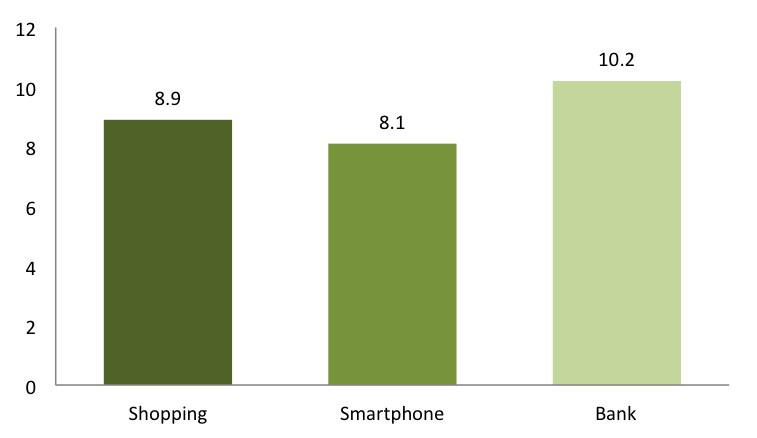
\includegraphics[width=0.45\textwidth]{pics/analysis/creationtime-gender-male.png}
        \label{fig:avgcreationtimemale}
      }
      \subfigure[Female]{
        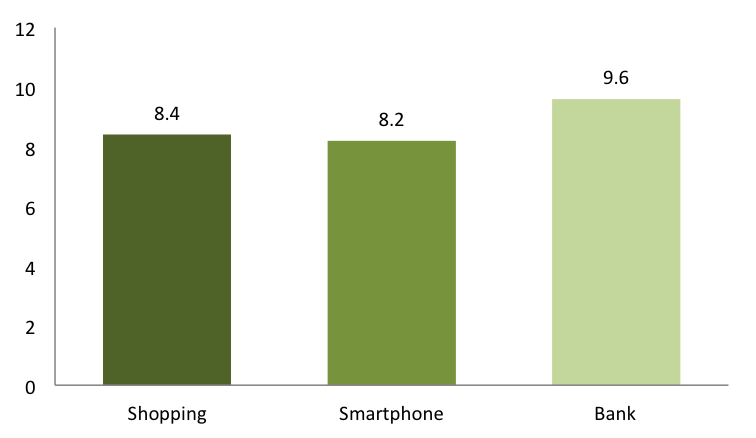
\includegraphics[width=0.45\textwidth]{pics/analysis/creationtime-gender-female.png}
        \label{fig:avgcreationtimefemale}
      }
      \caption{Average pattern creation time for gender}
      \label{fig:avgcreationtimegender}
    \end{figure}

    \clearpage
    \subsubsection{Average pattern length}
    Figure \ref{fig:avgpatternlengthmale} and \ref{fig:avgpatternlengthfemale} presents the average pattern length for patterns created by male and female participants, respectively. When looking at the patterns created shopping accounts and smartphones by male participants are having a slight difference in average length. The patterns created for smartphones have the lowest average pattern length of 5.47, while patterns have the longest average pattern length of 6.09. Female participants have roughly the same average length, 5.26 and 5.27, for patterns created for both shopping accounts and smartphones, respectively. The patterns created for banking accounts have the highest average length of 5.57. Comparing the average pattern length for patterns created by both genders, both genders have the longest length for banking account and the shortest average length created for smartphones. In general, the patterns created by male participants have an longer average length than patterns created by female participants. 

    \begin{figure}[H]
    	\centering
    	\subfigure[Male]{
    		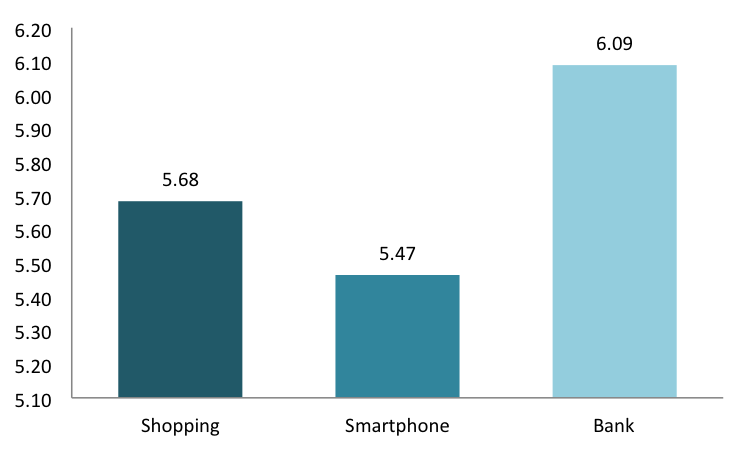
\includegraphics[width=0.45\textwidth]{pics/analysis/avgpatternlength-gender-male.png}
    		\label{fig:avgpatternlengthmale}
    	}
    	\subfigure[Female]{
    		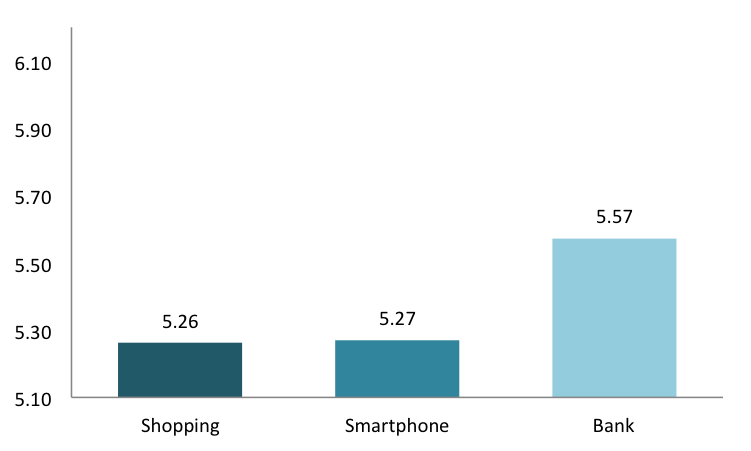
\includegraphics[width=0.45\textwidth]{pics/analysis/avgpatternlength-gender-female.png}
    		\label{fig:avgpatternlengthfemale}
    	}
    	\caption{Average pattern length for gender}
    	\label{fig:avgpatternlengthgender}
    \end{figure}

    Table \ref{tab:statsigLengthGender} summarizes the results when performing a two-tailed t-test for testing the difference in pattern length for patterns created by male and female respondents. The results reveal a significant difference in patterns created for shopping accounts and banking accounts. 

    \begin{table}[H]
      \centering
      \begin{tabular}{ c | c | c | c | c | c }
      \hline
        {\bf Pattern type} & {\bf Type} & {\bf Mean} & {\bf SD} & {\bf P-value} & {\bf Result} \\ \hline
        \multirow{2}{*}{Shopping}   & Male    & 5.68 & 1.76 & \multirow{2}{*}{0.00048841} & \multirow{2}{*}{\bf \color{olive}{Significant}} \\
                                    & Female  & 5.26 & 1.55 & & \\ \hline
        \multirow{2}{*}{Smartphone} & Male    & 5.47 & 1.60 & \multirow{2}{*}{0.08616198} & \multirow{2}{*}{\bf \color{red}{Not significant}} \\
                                    & Female  & 5.27 & 1.49 & & \\ \hline
        \multirow{2}{*}{Bank}       & Male    & 6.09 & 1.86 & \multirow{2}{*}{0.00009069} & \multirow{2}{*}{\bf \color{olive}{Significant}} \\
                                    & Female  & 5.57 & 1.72 & & \\ \hline
      \end{tabular}
      \caption{Statistical significance for pattern length and gender}
      \label{tab:statsigLengthGender}
    \end{table}

    \clearpage
    \subsubsection{Pattern length distribution}
    Figure \ref{fig:avgpatterndistgender} shows the pattern length distribution for both genders. The differences between the genders are noticeable in the endpoints, e.g. patterns with length 4 and 9. The male participants have a higher frequency of patterns with a longer length while the female participants have a higher frequency of patterns with a short length. The average number of patterns created with a length between 5 and 8 are about the same for both genders. 

    \begin{figure}[H]
    	\centering
    	\subfigure[Male]{
    		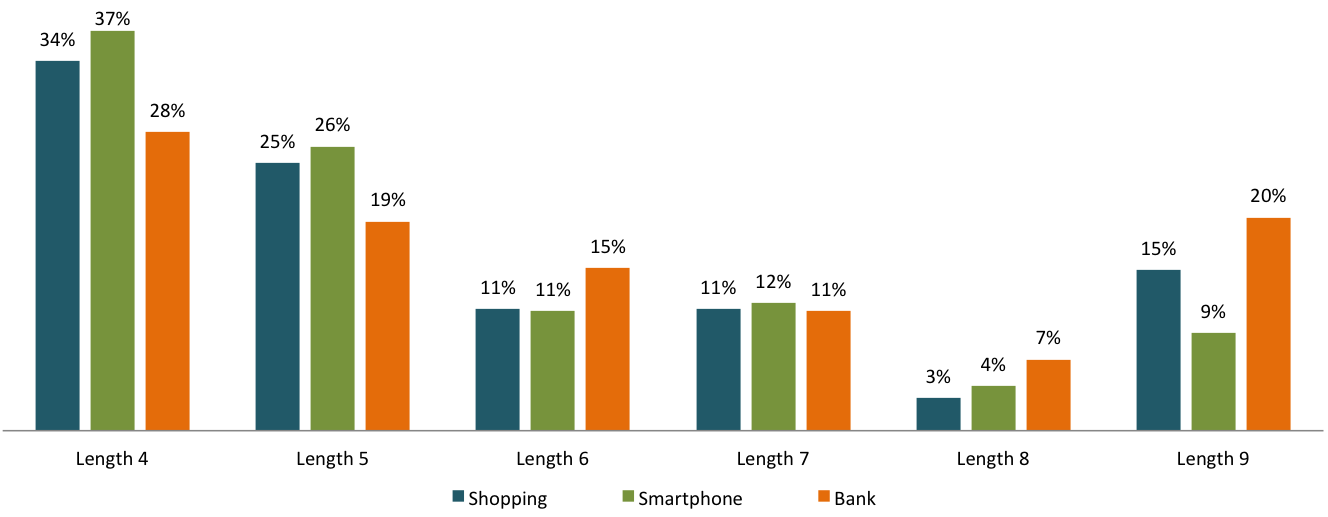
\includegraphics[width=1.0\textwidth]{pics/analysis/patterndist-gender-male.png}
    		\label{fig:avgpatternlengthdistmale}
    	}
    	\subfigure[Female]{
    		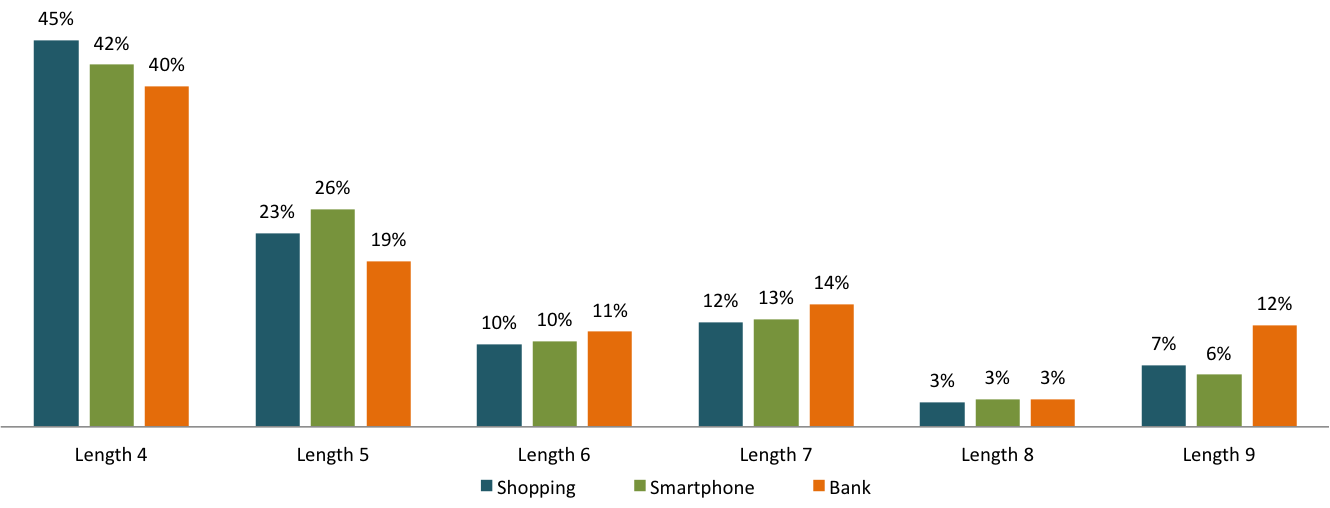
\includegraphics[width=1.0\textwidth]{pics/analysis/patterndist-gender-female.png}
    		\label{fig:avgpatternlengthdistfemale}
    	}
    	\caption{Average pattern length distribution for gender}
    	\label{fig:avgpatterndistgender}
    \end{figure}

    \clearpage
    \subsubsection{Pattern complexity}
    Table \ref{tab:gendertrength} summarizes the patterns strength for the three pattern types for both genders. Patterns created by female participants have the characteristics of infrequent use of both intersections and overlaps for all types. The patterns created for  smartphones by female respondents did not have a single pattern including an overlap, while only three patterns created by female respondents included an overlap.

    None of the patters created by female respondents reached the maximum strength score. The highest strength score reached for patterns created by female respondents was 40.072. The the patterns with the lowest pattern strength are patterns created for smartphones by female participants, only reaching a total strength score of 32.078. The patterns created by male respondents had a higher frequency of both intersections and overlaps, hence a higher average strength score for patterns created by male respondents. 

    \begin{table}[H]
      \centering
      \begin{tabular}{l || l | l || l | l || l | l }
        \hline
         & \multicolumn{2}{c||}{\bf Shopping} & \multicolumn{2}{c||}{\bf Smartphone} &\multicolumn{2}{c}{\bf Bank} \\ \hline
        {\bf Parameters}   & {\bf Male} & {\bf Female} & {\bf Male} & {\bf Female} & {\bf Male} & {\bf Female}\\ \hline
        \#Patterns         & 529    & 278    & 529    & 278    & 529    & 278    \\
        Avg. Size          & 5.684  & 5.263  & 5.465  & 5.270  & 6.089  & 5.572  \\
        Avg. Length        & 5.225  & 4.687  & 5.034  & 4.720  & 5.927  & 5.154  \\
        \#Intersections    & 147    & 20     & 120    & 23     & 284    & 69     \\
        Avg. Intersections & 0.278  & 0.072  & 0.227  & 0.082  & 0.537  & 0.248  \\
        \#Overlaps         & 13     & 1      & 12     & 0      & 16     & 3      \\
        Avg. Overlaps      & 0.025  & 0.04   & 0.023  & 0      & 0.030  & 0.011  \\ \hline
        Avg. Strength      & 14.127 & 12.062 & 13.221 & 12.122 & 16.398 & 13.744 \\ 
        Min strength       & 6.340  & 6.340  & 6.340  & 6.340  & 6.340  & 6.340  \\
        Max strength       & 44.442 & 32.950  & 44.442 & 32.078 & 44.442 & 40.072 \\ \hline
      \end{tabular}
      \caption{Pattern strength and gender}
      \label{tab:gendertrength}
    \end{table}

    Table \ref{tab:statsigComplexityGender} summarizes the results when performing a two-tailed t-test for testing the difference in pattern strength for patterns created by male and female respondents. The results reveal a significant difference in patterns created for all pattern types.

    \begin{table}[H]
      \centering
      \begin{tabular}{ c | c | c | c | c | c }
      \hline
        {\bf Pattern type} & {\bf Type} & {\bf Mean} & {\bf SD} & {\bf P-value} & {\bf Result} \\ \hline
        \multirow{2}{*}{Shopping}   & Male   & 14.13 & 8.02 & \multirow{2}{*}{0.00008596} & \multirow{2}{*}{\bf \color{olive}{Significant}} \\
                                    & Female & 12.06 & 6.48 & & \\ \hline
        \multirow{2}{*}{Smartphone} & Male   & 13.27 & 7.46 & \multirow{2}{*}{0.02153682} & \multirow{2}{*}{\bf \color{olive}{Significant}} \\
                                    & Female & 12.12 & 6.31 & & \\ \hline
        \multirow{2}{*}{Bank}       & Male   & 16.40 & 9.11 & \multirow{2}{*}{0.00001588} & \multirow{2}{*}{\bf \color{olive}{Significant}} \\
                                    & Female & 13.74 & 7.74 & & \\ \hline
      \end{tabular}
      \caption{Statistical significance for visual complexity and gender}
      \label{tab:statsigComplexityGender}
    \end{table}

	\subsection{Age}

    The participants are being divided into divided into seven age intervals; under 20, 20-24, 25-29, 30-34, 35-39, 40-49, and over 50. 

    \subsubsection{Average pattern creation time}
    Figure \ref{fig:patterncreationtimeage} is the graph visualizing the average creation time for each pattern type created by the different age groups. In general, patterns created for banking accounts have the highest average creation time across the various age groups. The average creation time seem to increase slightly as the age increases. It is noticeable that the creation time for smartphone patterns differs from the two other pattern types, especially for the younger participants where pattern creation time for smartphone are significantly lower. 

    %Figure: pattern creation time by gender
    \begin{figure}[H]
      \centering
      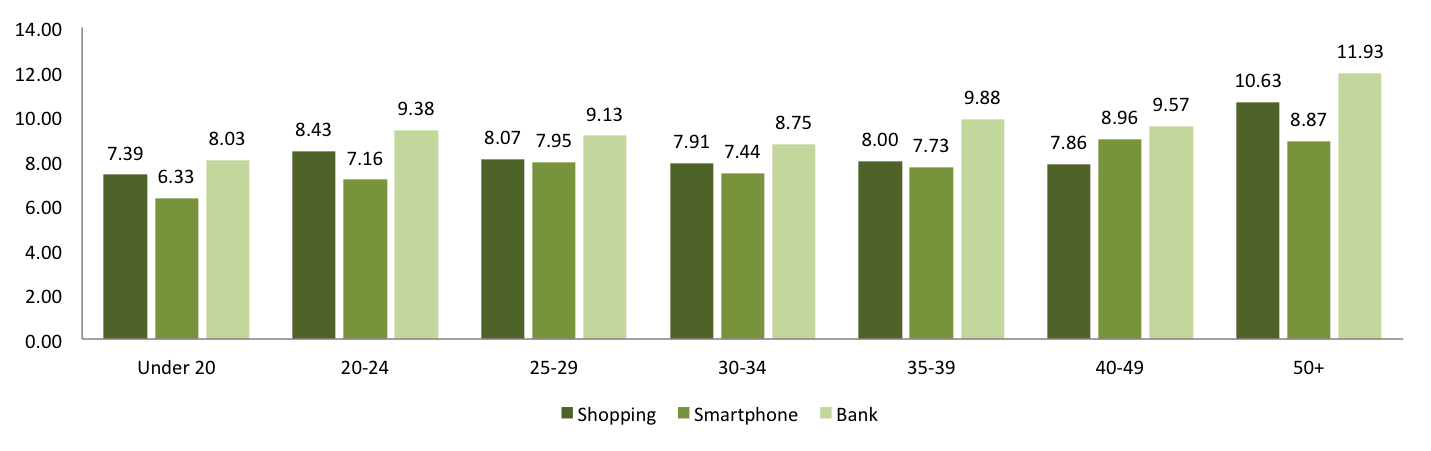
\includegraphics[width=\textwidth]{pics/analysis/creationtime-age.png}
      \caption{Pattern creation time by age}
      \label{fig:patterncreationtimeage}
    \end{figure}

    \clearpage
    \subsubsection{Average pattern length}
    Figure \ref{fig:patternlengthage} shows the pattern length for the three pattern types by the different age groups. In the graph, the average pattern length goes slightly down as the age increases. As the age increases, the average length of the all pattern types evens out. The age groups having the highest difference in pattern length is the patterns created by the youngest and the oldest respondents. 

    %Figure: Average pattern length by age
  	\begin{figure}[H]
	    \centering
	    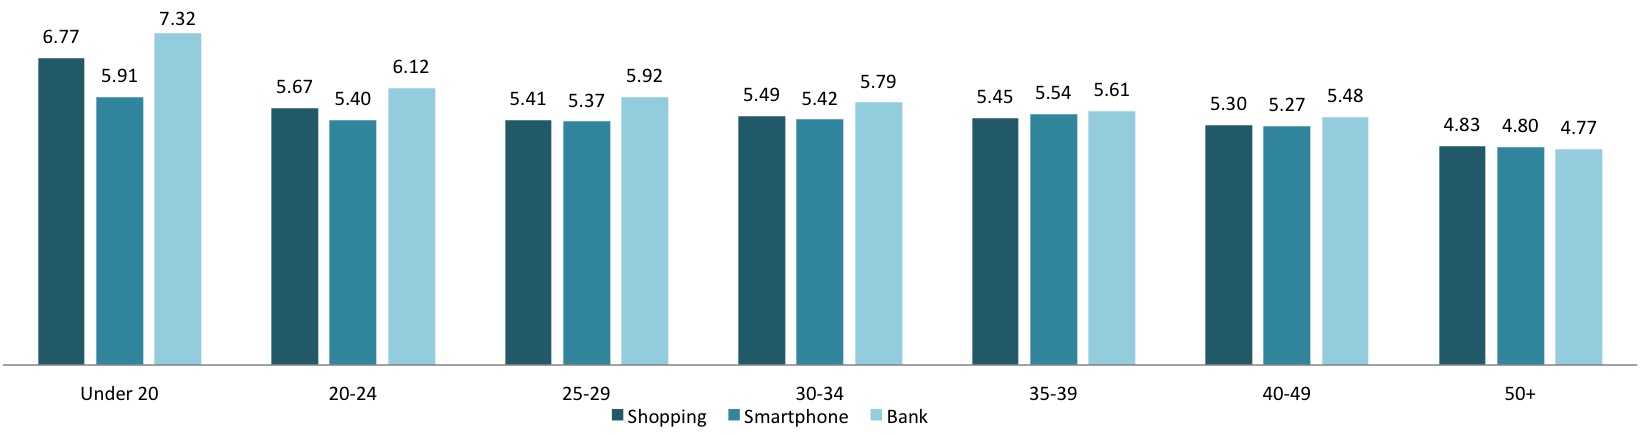
\includegraphics[width=\textwidth]{pics/analysis/avgpatternlength-age.png}
	    \caption{Pattern length by age}
	    \label{fig:patternlengthage}
  	\end{figure}

    Table \ref{tab:statsigLengthAge} summarizes the results when performing a two-tailed t-test for testing the difference in pattern length for patterns created by respondents with an age under 25 and respondents with a age of 25 years or older. The results reveal a significant difference in patterns created for shopping accounts and banking accounts. 

    \begin{table}[H]
      \centering
      \begin{tabular}{ c | c | c | c | c | c }
      \hline
        {\bf Pattern type} & {\bf Type} & {\bf Mean} & {\bf SD} & {\bf P-value} & {\bf Result} \\ \hline
        \multirow{2}{*}{Shopping}   & Under 25  & 5.74 & 1.76 & \multirow{2}{*}{0.00318325} & \multirow{2}{*}{\bf \color{olive}{Significant}} \\
                                    & 25+       & 5.38 & 1.64 & & \\ \hline
        \multirow{2}{*}{Smartphone} & Under 25  & 5.43 & 1.56 & \multirow{2}{*}{0.496001184} & \multirow{2}{*}{\bf \color{red}{Not significant}} \\
                                    & 25+       & 5.36 & 1.56 & & \\ \hline
        \multirow{2}{*}{Bank}       & Under 25  & 6.19 & 1.91 & \multirow{2}{*}{0.0001225} & \multirow{2}{*}{\bf \color{olive}{Significant}} \\
                                    & 25+       & 5.69 & 1.74 & & \\ \hline
      \end{tabular}
      \caption{Statistical significance for pattern length and age}
      \label{tab:statsigLengthAge}
    \end{table}

    \clearpage
    \subsubsection{Pattern complexity}
    The visual complexity of the patterns created by the different age groups are found in Table \ref{fig:strengthagedist}. To be able to illustrate the pattern strength for all age groups the data are shorten down to just visualize the pattern strength of each pattern type created by the different age groups. As mentioned earlier, the younger age respondents the longer patterns are created. The same is with the strength. The youngest age group have about twice as hight average pattern strength than the oldest age group. As the age increases, the strength of the different age groups also evens out. In general, bank have the highest average strength score while patterns created for smartphones have the lowest average strength score across the different age groups.

    %Figure: pattern strength based on age
    \begin{figure}[H]
      \centering
      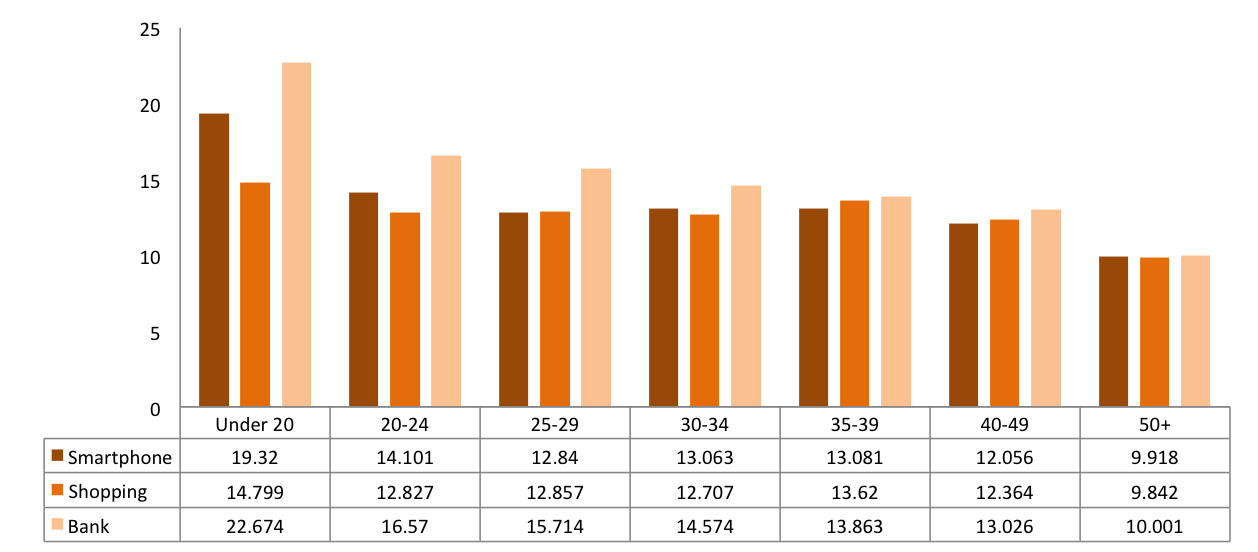
\includegraphics[width=\textwidth]{pics/analysis/strengthagedist.png}
      \caption{Pattern strength and age distribution}
      \label{fig:strengthagedist}
    \end{figure}

    Table \ref{tab:statsigComplexityAge} summarizes the results when performing a two-tailed t-test for testing the difference in pattern strength for patterns created by respondents with an age under 25 and respondents with a age of 25 years or older. The results reveal a significant difference in patterns created for shopping accounts and banking accounts. 

    \begin{table}[H]
      \centering
      \begin{tabular}{ c | c | c | c | c | c }
      \hline
        {\bf Pattern type} & {\bf Type} & {\bf Mean} & {\bf SD} & {\bf P-value} & {\bf Result} \\ \hline
        \multirow{2}{*}{Shopping}   & 14.43 & 8.14 & & \multirow{2}{*}{0.00089041} & \multirow{2}{*}{\bf \color{olive}{Significant}} \\
                                    & 12.61 & 7.00 & & & \\ \hline
        \multirow{2}{*}{Smartphone} & 12.95 & 6.88 & & \multirow{2}{*}{0.59266007} & \multirow{2}{*}{\bf \color{red}{Not significant}} \\
                                    & 12.68 & 7.10 & & & \\ \hline
        \multirow{2}{*}{Bank}       & 16.95 & 9.36 & & \multirow{2}{*}{0.00002946} & \multirow{2}{*}{\bf \color{olive}{Significant}} \\
                                    & 14.32 & 8.04 & & & \\ \hline
      \end{tabular}
      \caption{Statistical significance for visual complexity and age}
      \label{tab:statsigComplexityAge}
    \end{table}
         
	\subsection{Handedness}\label{sec:subgroupHandedness}
		% Kan her dra inn noe om hvilken hånd og finger som er brukt. 

    \subsubsection{Average pattern creation time}
    Figure \ref{fig:avgcreationtimehandedness} is the average creation time for patterns with respect to the handedness of the respondents. A participant can either be left or right handed. By looking at the graph, right-handed respondents has a lower average creation time than left-handed respondents. The only exception is the patterns created for smartphones where left-handed respondents have a slightly higher average creation time. For both left-handed and right-handed respondents, the average creation time for the banking account has the highest average creation among the three pattern types.  

      %Figure: Average pattern creation time for handednes
      \begin{figure}[H]
        \centering
        \subfigure[Right-handed]{
          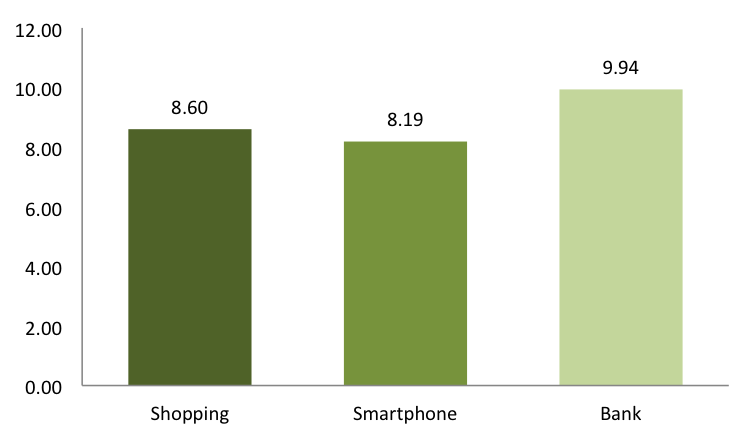
\includegraphics[width=0.45\textwidth]{pics/analysis/creationtime-handedness-right.png}
          \label{fig:avgcreationtimeright}
        }
        \subfigure[Left-handed]{
          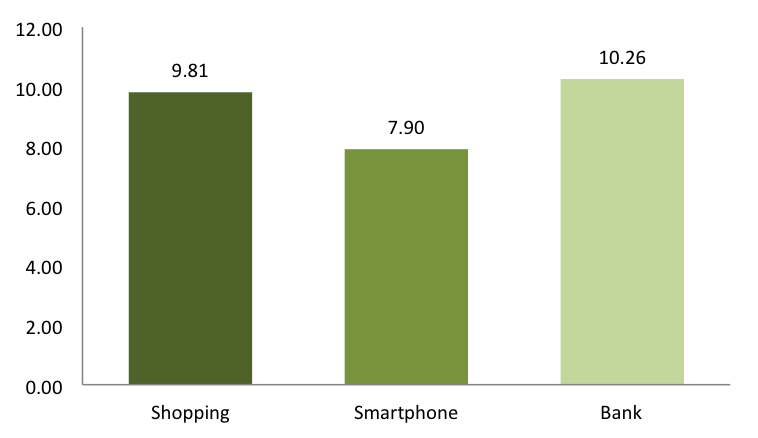
\includegraphics[width=0.45\textwidth]{pics/analysis/creationtime-handedness-left.png}
          \label{fig:avgcreationtimeleft}
        }
        \caption{Average pattern creation time for handedness}
        \label{fig:avgcreationtimehandedness}
      \end{figure}

    \subsubsection{Average pattern length}
    Figure \ref{fig:avgpatternlengthright} and \ref{fig:avgpatternlengthhandedness} presents the average pattern length for patterns created by left- and right-handed, respectively. In general, both left- and right-handed respondents have about the same average pattern length. One exception is the patterns created for smartphones where there is a slight indication of left-handed people creating shorter patterns than right-handed people. The average pattern length for patterns created for smartphones created by right- and left-handed respondents are 5.42 and 5.28 respectively. The patterns that are getting the highest average length is the patterns created for banking accounts with an average pattern length of 5.93 and 5.90 for right- and left-handed respondents respectiveley. 

      %Figure: Average pattern length for handedness
      \begin{figure}[H]
      	\centering
      	\subfigure[Right-handed]{
      		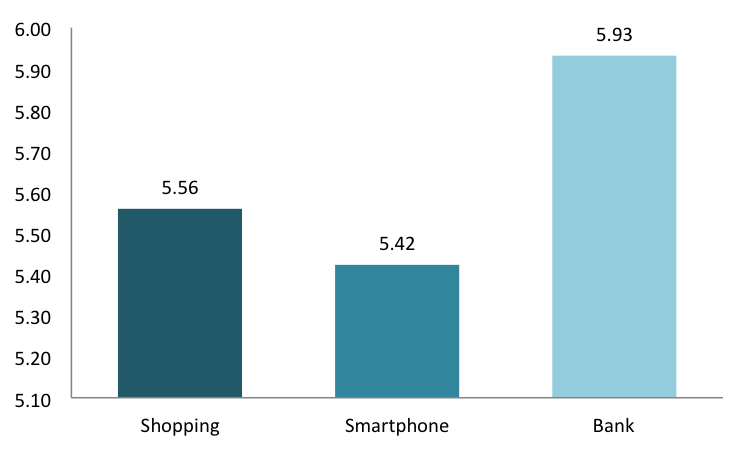
\includegraphics[width=0.45\textwidth]{pics/analysis/avgpatternlength-handedness-right.png}
      		\label{fig:avgpatternlengthright}
      	}
      	\subfigure[Left-handed]{
      		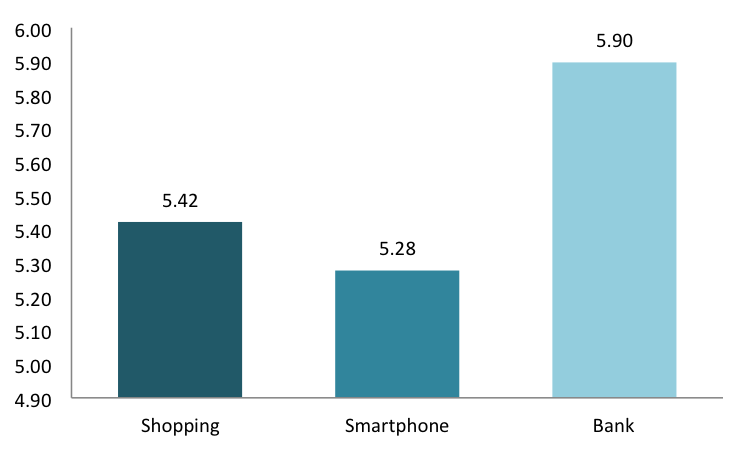
\includegraphics[width=0.45\textwidth]{pics/analysis/avgpatternlength-handedness-left.png}
      		\label{fig:avgpatternlengthleft}
      	}
      	\caption{Average pattern length for handedness}
      	\label{fig:avgpatternlengthhandedness}
      \end{figure}

    Table \ref{tab:statsigLengthHandedness} summarizes the results when performing a two-tailed t-test for testing the difference in pattern length for patterns created by left- and right-handed respondents. The results reveal no significant differences for any of the pattern types.

    \begin{table}[H]
      \centering
      \begin{tabular}{ c | c | c | c | c | c }
      \hline
        {\bf Pattern type} & {\bf Type} & {\bf Mean} & {\bf SD} & {\bf P-value} & {\bf Result} \\ \hline
        \multirow{2}{*}{Shopping}   & Left  & 5.42 & 1.75 & \multirow{2}{*}{0.47066079} & \multirow{2}{*}{\bf \color{red}{Not significant}} \\
                                    & Right & 5.56 & 1.70 & & \\ \hline
        \multirow{2}{*}{Smartphone} & Left  & 5.28 & 1.60 & \multirow{2}{*}{0.40381003} & \multirow{2}{*}{\bf \color{red}{Not significant}} \\
                                    & Right & 5.42 & 1.56 & & \\ \hline
        \multirow{2}{*}{Bank}       & Left  & 5.90 & 1.99 & \multirow{2}{*}{0.86996995} & \multirow{2}{*}{\bf \color{red}{Not significant}} \\
                                    & Right & 6.93 & 1.81 & & \\ \hline
      \end{tabular}
      \caption{Statistical significance for pattern length and handedness}
      \label{tab:statsigLengthHandedness}
    \end{table}

    \subsubsection{Pattern length distribution}
    Figure \ref{fig:avgpatterndisthandedness} shows the pattern length distribution for both right- and left-handed respondents. The selection of pattern length seems to have no significant difference beside left-handed respondents having a tendency of having more patterns of length 4 than than right-handed respondents. It is also noticeable that the frequency of patterns tends to go down as the pattern length goes up. The only exception are patterns with length 8 where patterns with length 7 and 9 have a higher frequency.

    A pattern length of 4 and 5 can be considered as a short pattern, whereas the minimum pattern length for Android Pattern Lock is 4. By looking at the number of patterns with the minimum length, 45\% of the left-handed respondents created a pattern of length 4 for smartphones. In total, 70\% of all left-handed respondent created a pattern of length 4 or 5 for smartphones while 65\% of the patterns created for smartphones by Right-handed respondents is of length 4 or 5. Compared to patterns created for banking accounts, there are only 51\% and 52\% of the patterns having a length of 4 or 5 for right- and left-handed respondents, respectively. This resulr in a difference of 15\% and 20\% for right- and left-handed respondents between patterns created for smartphone and banking accounts of length 4 and 5.

      %Figure: Pattern length dist handedness
      \begin{figure}[H]
      	\centering
      	\subfigure[Right-handed]{
      		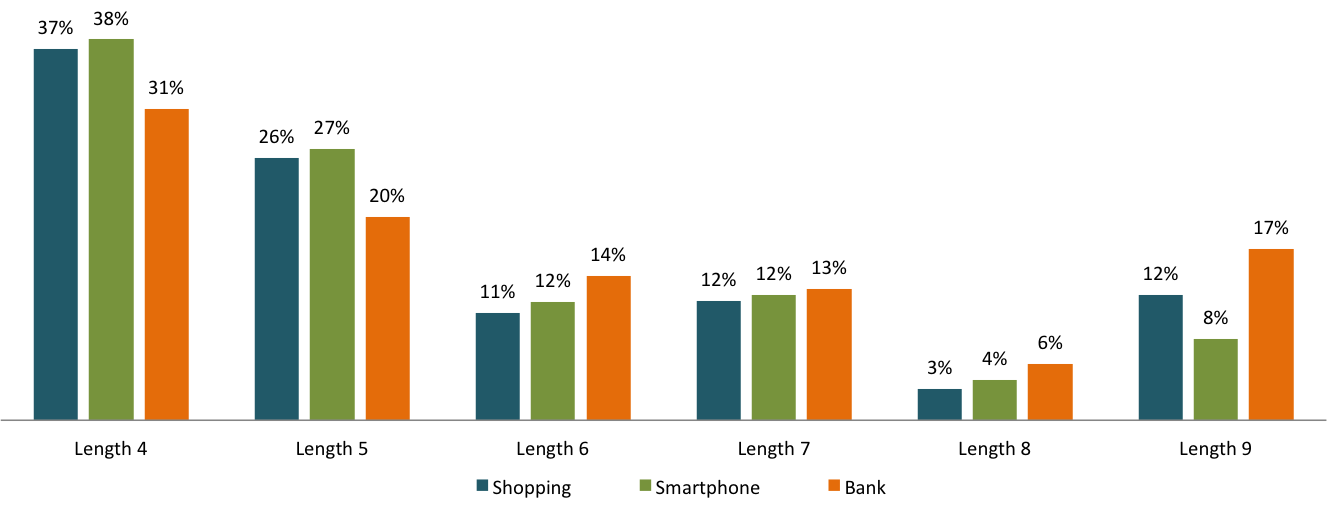
\includegraphics[width=1.0\textwidth]{pics/analysis/patterndist-handedness-right.png}
      		\label{fig:avgpatternlengthdistright}
      	}
      	\subfigure[Left-handed]{
      		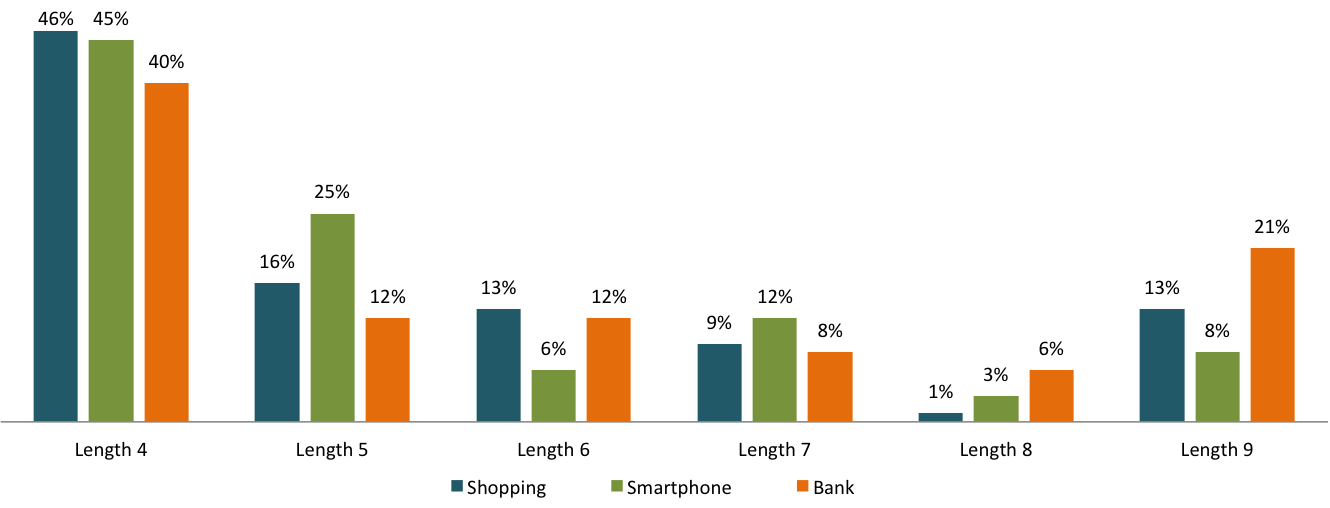
\includegraphics[width=1.0\textwidth]{pics/analysis/patterndist-handedness-left.png}
      		\label{fig:avgpatternlengthdistleft}
      	}
      	\caption{Average pattern length distribution for handedness}
      	\label{fig:avgpatterndisthandedness}
      \end{figure}

    \subsubsection{Pattern complexity}
    Table \ref{tab:handednessstrength} is the pattern strength for each pattern type with respect to the handedness of the respondents. The table does also include an overview of the parameters used for calculating the pattern strength. 

    The number of intersections differs on both shopping account and smartphone when comparing the patterns created by left- and right-handed respondents. The only pattern type having an equal number of intersections between right- and left-handed respondents are patterns created for banking accounts, resulting in 0.443 and 0.433 average number of intersections. Left-handed respondents have approximately an equal number of intersections for both shopping and bank, but only half the number half as many intersections for patterns created for smartphones. Patterns created by right-handed respondents has an approximately equal distribution of intersections on patterns created for shopping account and smartphones, but about twice as many occurrences of intersections on patterns created for banking accounts.

    Comparing the number of overlaps, left-handed respondents have only one occurrence of overlap in one of the patterns created for banking accounts. Right-handed respondents have a somewhat higher number of overlaps, but overlaps still rarely occur. The pattern type reaching the highest number of overlaps and intersections are the patterns created for banking accounts.

    By comparing average strength for both right- and left-handed respondents, the strength is roughly the same. In general, pattern strength has an indication to be higher for patterns created for banking accounts, but there are no significant differences caused by handedness. Looking at the maximum pattern strength reached, both right- and left-handed respondents had reached a maximum pattern strength of 44.441 that is the same as the maximum pattern strength in the entire dataset. For patterns created for smartphones, the maximum strengths for both right- and left-handed respondents were 43.187 and 37.280 respectiveley. 

      %Table: Pattern strength handedness
      \begin{table}[H]
        \centering
        \begin{tabular}{l || l | l || l | l || l | l }
          \hline
           & \multicolumn{2}{c||}{\bf Shopping} & \multicolumn{2}{c||}{\bf Smartphone} &\multicolumn{2}{c}{\bf Bank} \\ \hline
          {\bf Parameters}   & {\bf Right} & {\bf Left} & {\bf Right} & {\bf Left} & {\bf Right} & {\bf Left}\\ \hline
          \#Patterns         & 690    & 97      & 690     & 97      & 690    & 97     \\
          Avg. Size          & 5.560  & 5.423   & 5.423   & 5.280   & 5.932  & 5.897  \\
          Avg. Length        & 5.036  & 5.134   & 4.966   & 4.781   & 5.703  & 5.566  \\
          \#Intersections    & 126    & 42      & 124     & 18      & 306    & 42     \\
          Avg. Intersections & 0.183  & 0.433   & 0.180   & 0.186   & 0.443  & 0.433  \\
          \#Overlaps         & 14     & 0       & 12      & 0       & 18     & 1      \\
          Avg. Overlaps      & 0.020  & 0.0     & 0.017   & 0.0     & 0.026  & 0.010  \\ \hline
          Avg. Strength      & 13.455 & 13.360  & 12.966  & 12.339  & 15.601 & 15.339 \\ 
          Min strength       & 6.340  & 6.340   & 6.340   & 6.340   & 6.340  & 6.340  \\
          Max strength       & 39.827 & 44.441  & 43.187  & 37.280  & 44.441 & 44.441 \\ \hline
        \end{tabular}
        \caption{Pattern strength and handedness}
        \label{tab:handednessstrength} 
      \end{table}

      
      Table \ref{tab:statsigComplexityHandedness} summarizes the results when performing a two-tailed t-test for testing the difference in pattern strength for patterns created by left- and right-handed respondents. The results reveal no significant differences for any of the pattern types. 

      \begin{table}[H]
      \centering
        \begin{tabular}{ c | c | c | c | c | c }
        \hline
          {\bf Pattern type} & {\bf Type} & {\bf Mean} & {\bf SD} & {\bf P-value} & {\bf Result} \\ \hline
          \multirow{2}{*}{Shopping}   & Left  & 13.36 & 8.64 & \multirow{2}{*}{0.9176142} & \multirow{2}{*}{\bf \color{red}{Not significant}} \\
                                      & Right & 13.46 & 7.46 & & \\ \hline
          \multirow{2}{*}{Smartphone} & Left  & 12.34 & 7.29 & \multirow{2}{*}{0.4271685} & \multirow{2}{*}{\bf \color{red}{Not significant}} \\
                                      & Right & 12.97 & 7.03 & & \\ \hline
          \multirow{2}{*}{Bank}       & Left  & 15.34 & 9.50 & \multirow{2}{*}{0.7970912} & \multirow{2}{*}{\bf \color{red}{Not significant}} \\
                                      & Right & 15.60 & 8.67 & & \\ \hline
        \end{tabular}
        \caption{Statistical significance for visual complexity and handedness}
        \label{tab:statsigComplexityHandedness}
      \end{table}

    \clearpage
    \subsubsection{Typing habits}
    Handedness is a human characteristic influencing the physical interaction with a smartphone, hence might having an impact on the way a person create a pattern. The only way a person are interacting with a smartphone is by using their hands, making this an important behavior to study. The hand used are also being defined by handedness, making it interesting to look at the typing behavior of both. 

    Table \ref{tab:righthandfinger} and \ref{tab:lefthandfinger} summarizes the typing habits of the respondents focusing on the physical interaction with the touch screen. The parameters included are handedness, hand used to hold the smartphone, and the finger used to type the pattern. Table \ref{tab:righthandfinger} are summarizing the typing habits of right-handed respondents while Table \ref{tab:lefthandfinger} are summarizing the typing habits of left-handed respondents.

    The two main options for interacting with a smartphone are described in Section \ref{sec:thecreatedpatterns}. By starting looking at the right-handed respondents, the majority (53\%) are interacting with the screen as described in category 1. This means that the 53\% of the right-handed respondents used their right hand and their thumb, e.g. used only one hand, for interacting with the screen. About 32\% of the right-handed respondents interacted with the screen as described in category 2. In other words, 32\% of the right-handed respondents used their left hand to hold the smartphone while using their forefinger on their right hand for interacting with the screen. The last 15\% of the right-handed respondents had other typing habits than the two most common ways of interacting with the screen.

    The left-handed respondents had a more indefinite typing habit because none of the alternatives appear to be more common than others. By summarizing the numbers, it seems that the frequency of category 1 and 2 for left-handed respondents have no significant difference in number of respondents.  26 respondents are in category 1 and 26 respondents are in category 2. Another observation is that 22 of the left-handed respondents interact in the same way as Category 1 for right-handed respondents. Only 5\% of the right-handed respondents acts in the same way as Category 1 for left-handed respondents. In other words, the typing habits of right-handed respondents seems to be more predictable than as for the typing habits of left-handed respondents.

  		%Table: typing habits, handedness
      \begin{table}[H]
        \parbox{.5\linewidth}{
          \centering
          \begin{tabular}{ l | l | l }
            \hline
            {\bf Hand used} & {\bf Finger used} & {\bf \#} \\ \hline
            \multirow{3}{*}{Right hand} & Thumb & 366 \\
            & Forefinger & 41 \\
            & Other & 8 \\ \hline
            \multirow{3}{*}{Left hand} & Thumb & 33 \\
            & Forefinger & 217 \\
            & Other & 23 \\ \hline
          \end{tabular}
          \caption{{\bf Right-handed} typing habits}
          \label{tab:righthandfinger}
        }
        \hfill
        \parbox{.5\linewidth}{
          \centering
          \begin{tabular}{ l | l | l }
            \hline
            {\bf Hand used} & {\bf Finger used} & {\bf \#} \\ \hline
            \multirow{3}{*}{Right hand} & Thumb & 22 \\ 
            & Forefinger & 26 \\
            & Other & 6 \\ \hline
            \multirow{3}{*}{Left hand} & Thumb & 26 \\ 
            & Forefinger & 10 \\
            & Other & 4 \\ \hline
          \end{tabular}
          \caption{{\bf Left-handed} typing habits}
          \label{tab:lefthandfinger}
        }
      \end{table}

    \clearpage
    \subsubsection{Bias in the Selection of Start Node}
    How a person are holding a smartphone might impact the nodes being reachable. It is defined two main types of typing a pattern, e.g. either use one or both hands. When using both hands, one hand are used to hold the phone while the other hand are used for interacting with the screen. When holding the smartphone in one hand, the same hand are used for both holding and interacting with the screen, whereas the thumb are the only finger available when using one hand. Figure \ref{fig:handednessstartingpoint} are showing likelihood of starting nodes from patterns created by respondents with different dominant hand, combined with the two ways of holding a smartphone and finger used. Figure \ref{fig:handednessstartingpoint1} and \ref{fig:handednessstartingpoin2} are looking at right-handed respondents' selection in starting node for patterns created by using either one or two hands, respectively. 

    Figure \ref{fig:handednessstartingpoint1} are showing the choice of starting nodes for patterns created by right-handed respondents holding the smartphone in the right hand using the thumb on the same hand for pattern creation. As seen in Figure \ref{fig:startingNode4}, node 1, 3, 7 are the most common choice for selecting starting node. Figure \ref{fig:handednessstartingpoin2} are the selection of starting node by right-handed respondents using their left hand holding the smartphone using their right forefinger for pattern creation. The three main starting nodes are 1, 3, and 7, similarly for the right-handed respondents using one hand. 

    Figure \ref{fig:handednessstartingpoint3} are showing the selection of starting nodes for patterns created by left-handed respondents holding the smartphone in the left hand using the thumb on the same hand for pattern creation. About 54\% of the left-handed respondents using one hand starting their pattern in node 1. The majority of the left-handed respondents using one hand starts their pattern on the left side of the grid. The nodes in Figure \ref{fig:handednessstartingpoint4} are starting points selected by left-handed respondents using the right hand for holding the smartphone while interacting with the screen using the forefinger on the left hand. 

    By comparing handedness and way of creating the patterns, the way of holding the smartphone, either using one or two hands, do not seem to affect the node starting node. For all ways of creating a pattern with respect to handedness, the majority of the patterns are created by starting on the left side of the grid.

      \clearpage

      \begin{figure}[H]
        \vspace{1.5cm}
        \centering
        \subfigure[Patterns created by right-handed respondents holding the smartphone in the right hand using the thumb on the same hand]{
          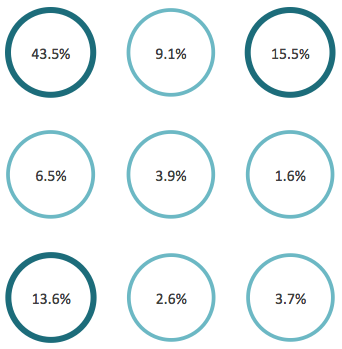
\includegraphics[width=0.45\textwidth]{pics/analysis/RRT.png}
          \label{fig:handednessstartingpoint1}
        }
        \hspace{0.5cm}
        \subfigure[Patterns created by right-handed respondents holding the smartphone in the left hand using the forefinger on the left hand]{
          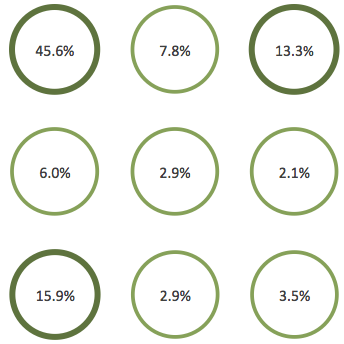
\includegraphics[width=0.45\textwidth]{pics/analysis/RLF.png}
          \label{fig:handednessstartingpoin2}
        }
        \subfigure[Patterns created by left-handed respondents holding the smartphone in the left hand using the thumb on the same hand]{
          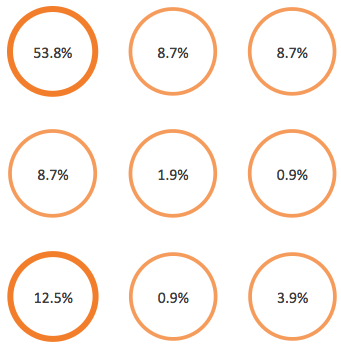
\includegraphics[width=0.45\textwidth]{pics/analysis/LLT.png}
          \label{fig:handednessstartingpoint3}
        }
        \hspace{0.5cm}
        \subfigure[Patterns created by left-handed respondents holding the smartphone in the right hand using the forefinger on the left hand]{
          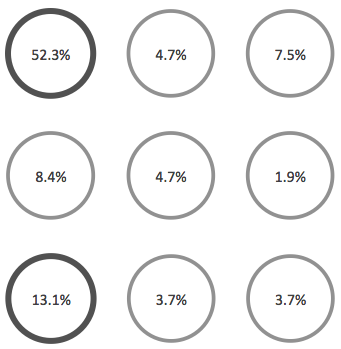
\includegraphics[width=0.45\textwidth]{pics/analysis/LRF.png}
          \label{fig:handednessstartingpoint4}
        }
        \caption{Starting node based on handedness, hand used to hold smartphone, and finger used used when creating patterns}
        \label{fig:handednessstartingpoint}
      \end{figure}

  \clearpage
	\subsection{Experience with IT and Security}

    This section takes a more detailed review of the patterns created by people with a difference in experience with IT and security. The level of interest, and experience with IT and security, can cause people to create different passwords due to risk perception and security awareness.  

    \subsubsection{Average pattern creation time}
    Figure \ref{fig:avgcreationtimeexperience} is showing the average creation time measured in seconds for both respondents experienced and not experienced with IT and security. 

    Figure \ref{fig:avgcreationtimeyes} are showing the average creation time for the three pattern types created by respondents experienced with IT and security. The patterns with the highest creation time are the patterns created for banking accounts with an average creation time of 9.42 seconds. The patterns with the lowest average creation time are being created for smartphones with an average creation time of 7.75 seconds. 

    Figure \ref{fig:avgcreationtimeno} are showing the average creation time for the three pattern types created by respondents inexperienced with IT and security. The patterns with the highest creation time are the patterns created for banking accounts with an average creation time of 9.29 seconds. The patterns with the lowest average creation time are being created for smartphones with an average creation time of 7.42 seconds.

    Comparing the respondents experienced and inexperienced with IT and security, the inexperienced respondents has a slightly slower response time for pattern creation for all three pattern types. 

      %Figure: Average pattern creation time for Experience
      \begin{figure}[H]
        \centering
        \subfigure[Experience with IT and security]{
          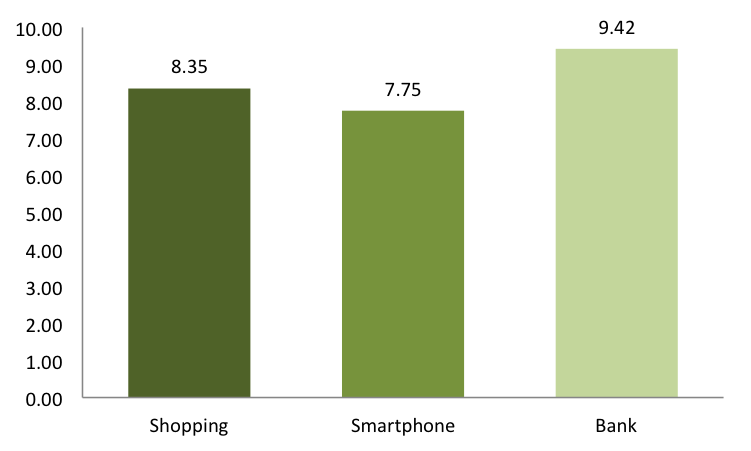
\includegraphics[width=0.45\textwidth]{pics/analysis/creationtime-experience-yes.png}
          \label{fig:avgcreationtimeyes}
        }
        \subfigure[No experience with IT and security]{
          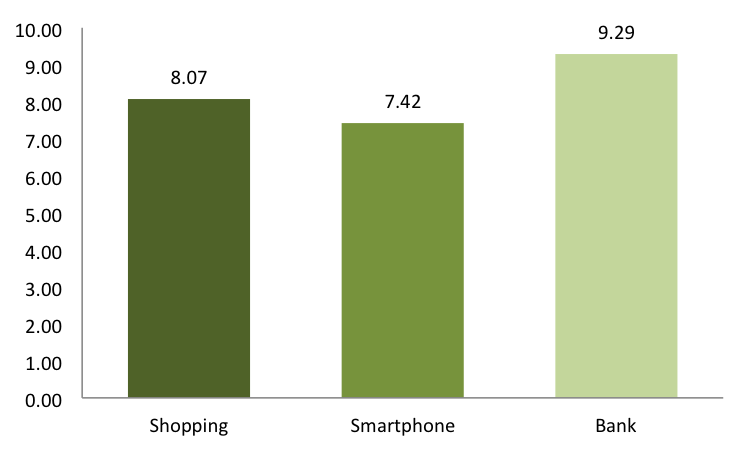
\includegraphics[width=0.45\textwidth]{pics/analysis/creationtime-experience-no.png}
          \label{fig:avgcreationtimeno}
        }
        \caption{Average pattern creation time for experience with IT and security}
        \label{fig:avgcreationtimeexperience}
      \end{figure}

    \clearpage
    \subsubsection{Average pattern length}
    Figure \ref{fig:avgpatternlengthyes} are showing the average pattern length for patterns created by respondents experienced with IT and security. The patterns with the highest average pattern length are being created for banking accounts with a total average pattern length of 6.11. The pattern type with the shortest average pattern length are patterns created for smartphones with an average pattern length of 5.48. Figure \ref{fig:avgpatternlengthfeno} are showing the average pattern length for patterns created by respondents inexperienced with IT and security. The patterns with the highest average pattern length are being created for banking accounts with a total average pattern length of 5.61. The pattern type with the shortest average pattern length are patterns created for smartphones with an average pattern length of 5.27. 

    The trends in the graphs show that respondents with experience in IT and security create longer patterns than people inexperienced with IT and security for all three pattern types. For both graphs, patterns created for banking accounts has the highest average length while patterns created for smartphones have the shortest average pattern length. 

      %Figure: Average pattern length for experience
      \begin{figure}[H]
        \centering
        \subfigure[Experience with IT and security]{
          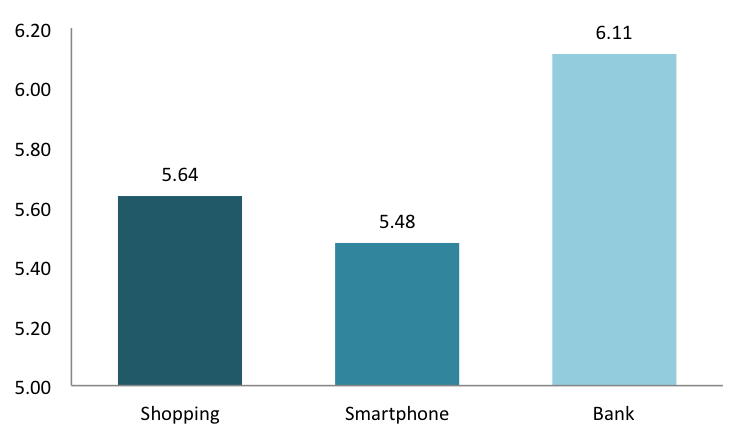
\includegraphics[width=0.45\textwidth]{pics/analysis/avgpatternlength-experience-yes.png}
          \label{fig:avgpatternlengthyes}
        }
        \subfigure[No experience with IT and security]{
          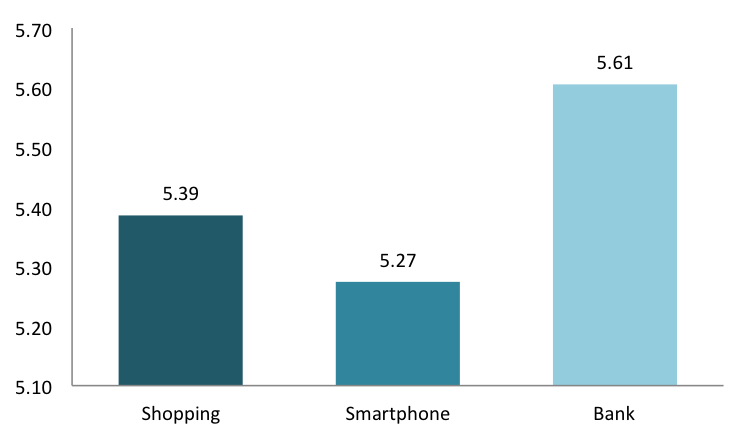
\includegraphics[width=0.45\textwidth]{pics/analysis/avgpatternlength-experience-no.png}
          \label{fig:avgpatternlengthfeno}
        }
        \caption{Average pattern length for experience with IT and security}
        \label{fig:avgpatternlengthexperience}
      \end{figure}

    Table \ref{tab:statsigLengthExperience} summarizes the results when performing a two-tailed t-test for testing the difference in pattern length for patterns created by respondents being experienced and inexperienced with IT and security. The results reveal a significant difference in patterns created for banking accounts. 

    \begin{table}[H]
      \centering
      \begin{tabular}{ c | c | c | c | c | c }
      \hline
        {\bf Pattern type} & {\bf Type} & {\bf Mean} & {\bf SD} & {\bf P-value} & {\bf Result} \\ \hline
        \multirow{2}{*}{Shopping}   & Experienced   & 5.64 & 1.72 & \multirow{2}{*}{0.038204664} & \multirow{2}{*}{\bf \color{red}{Not significant}} \\
                                    & Inexperienced & 5.39 & 1.66 & & \\ \hline
        \multirow{2}{*}{Smartphone} & experienced   & 5.48 & 1.60 & \multirow{2}{*}{0.064560991} & \multirow{2}{*}{\bf \color{red}{Not significant}} \\
                                    & Inexperienced & 5.27 & 1.50 & & \\ \hline
        \multirow{2}{*}{Bank}       & Experienced   & 6.11 & 1.86 & \multirow{2}{*}{0.000083188} & \multirow{2}{*}{\bf \color{olive}{Significant}} \\
                                    & Inexperienced & 5.61 & 1.74 & & \\ \hline
      \end{tabular}
      \caption{Statistical significance for pattern length and experience with IT and security}
      \label{tab:statsigLengthExperience}
    \end{table}

    \subsubsection{Pattern length distribution}
    Figure \ref{fig:avgpatternlengthdistyes} is the distribution of pattern length for patterns created by respondents experienced with IT and security. For the patterns created for smartphones, 70\% of the patterns constitutes of patterns with a lower length, e.g. patterns with a length between 4 and 6. For patterns created for banking accounts, 62\% of the patterns are created having a low length. The created patterns having a length of 9 nodes are the patterns created for banking accounts. Figure \ref{fig:avgpatternlengthdistno} is the pattern length distribution of patterns created by respondents inexperienced with IT and security. For the patterns created for smartphones, 79\% of the patterns are patterns having a low length.

    By comparing the pattern length distribution for experienced and inexperienced respondents, the patterns created by inexperienced respondents have a higher frequency of patterns with lower pattern length than patterns created by experienced respondents. The difference observed is that experienced respondents create fewer patterns of low length for banking accounts compared to inexperienced respondents. Instead of having a high frequency of short patterns, patterns created by experienced respondents have a higher frequency of patterns with length 9 for banking accounts. Experienced users do only have 27\% of their patterns for banking accounts created with the length 4, while inexperienced users have 39\% of their patterns for banking accounts created with the length 4. Both graphs show that the lower the length a lower frequency of the pattern length occurs.

      %Figure: Average pattern length distribution for experience
      \begin{figure}[H]
        \centering
        \subfigure[Experience with IT and security]{
          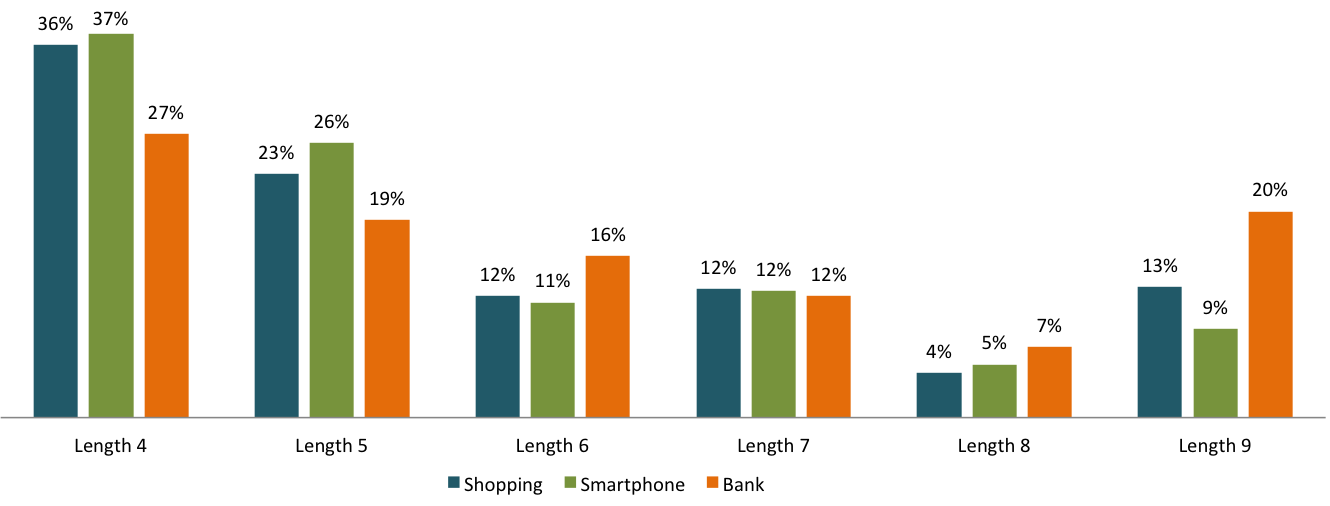
\includegraphics[width=1.0\textwidth]{pics/analysis/patterndist-experience-yes.png}
          \label{fig:avgpatternlengthdistyes}
        }
        \subfigure[No experience with IT and security]{
          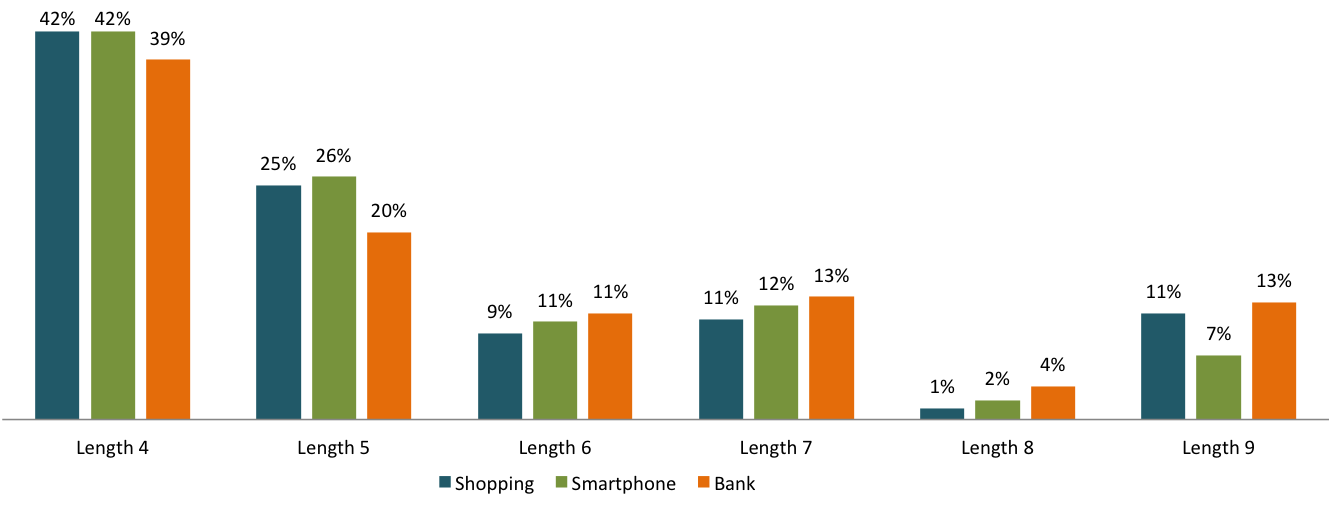
\includegraphics[width=1.0\textwidth]{pics/analysis/patterndist-experience-no.png}
          \label{fig:avgpatternlengthdistno}
        }
        \caption{Average pattern length distribution for experience with IT and security}
        \label{fig:avgpatterndistexperience}
      \end{figure}

    \clearpage
    \subsubsection{Pattern complexity}
    Table \ref{tab:experiencestrength} is a summary of the parameters used for calculating the pattern strength for each pattern type with respect to the respondents experience with IT and security. 

    Patterns created by experienced users seems to have a higher frequency of both overlaps and intersections, hence reaching a higher average strength score for all patterns created by experienced respondents. The patterns created for smartphones, by both experienced and inexperienced respondents, was the patterns getting the lowest strength score. 

    By comparing average strength for both experienced and inexperienced respondents, the patterns created by experienced respondents have obtained the highest average strength. Looking at the maximum pattern strength, neither the experienced or the inexperienced respondents manage to create a pattern reaching the maximum pattern score for the dataset.

      %Table: Password strength and Experience with IT/Security
      \begin{table}[H]
        \centering
        \begin{tabular}{l || l | l || l | l || l | l }
          \hline
           & \multicolumn{2}{c||}{\bf Shopping} & \multicolumn{2}{c||}{\bf Smartphone} &\multicolumn{2}{c}{\bf Bank} \\ \hline
          {\bf Parameters}   & {\bf Yes} & {\bf No} & {\bf Yes} & {\bf No} & {\bf Yes} & {\bf No}\\ \hline
          \#Patterns         & 470    & 332    & 470    & 332    & 470    & 332    \\
          Avg. Size          & 5.636  & 5.386  & 5.479  & 5.274  & 6.113  & 5.605  \\
          Avg. Length        & 5.182  & 4.818  & 5.045  & 4.753  & 5.919  & 5.281  \\
          \#Intersections    & 123    & 41     & 108    & 34     & 231    & 121    \\
          Avg. Intersections & 0.262  & 0.123  & 0.230  & 0.102  & 0.491  & 0.364  \\
          \#Overlaps         & 10     & 4      & 9      & 3      & 13     & 6      \\
          Avg. Overlaps      & 0.021  & 0.012  & 0.019  & 0.009  & 0.028  & 0.018  \\ \hline
          Avg. Strength      & 13.911 & 12.635 & 13.271 & 12.202 & 16.417 & 14.089 \\ 
          Min strength       & 6.340  & 6.340  & 6.340  & 6.340  & 6.340  & 6.340  \\
          Max strength       & 44.441 & 39.827 & 43.187 & 38.870 & 44.441 & 44.441 \\ \hline
        \end{tabular}
        \caption{Password strength and Experience with IT/Security}
        \label{tab:experiencestrength} 
      \end{table} 

    Table \ref{tab:statsigComplexityExperience} summarizes the results when performing a two-tailed t-test for testing the difference in pattern strength for patterns created by respondents being experienced and inexperienced with IT and security. The results reveal a significant difference in patterns created for all three pattern types.

    \begin{table}[H]
    \centering
      \begin{tabular}{ c | c | c | c | c | c }
      \hline
        {\bf Pattern type} & {\bf Type} & {\bf Mean} & {\bf SD} & {\bf P-value} & {\bf Result} \\ \hline
        \multirow{2}{*}{Shopping}   & Experienced   & 13.91 & 7.78 & \multirow{2}{*}{0.01699014} & \multirow{2}{*}{\bf \color{olive}{Significant}} \\
                                    & Inexperienced & 12.64 & 7.19 & & \\ \hline
        \multirow{2}{*}{Smartphone} & Experienced   & 13.32 & 7.40 & \multirow{2}{*}{0.02375298} & \multirow{2}{*}{\bf \color{olive}{Significant}} \\
                                    & Inexperienced & 12.20 & 6.52 & & \\ \hline
        \multirow{2}{*}{Bank}       & Experienced   & 16.42 & 8.94 & \multirow{2}{*}{0.00015740} & \multirow{2}{*}{\bf \color{olive}{Significant}} \\
                                    & Inexperienced & 14.09 & 8.26 & & \\ \hline
      \end{tabular}
      \caption{Statistical significance for visual complexity and experience with IT and security}
      \label{tab:statsigComplexityExperience}
    \end{table}

  \subsection{Hand Size and Screen Size}\label{sec:classificationhandsizescreensize}
    To be able to analyze if there is a correlation between hand size and choice of graphical patterns, the data collected needs to be validated due to the subjective form. Along with the hand size, the screen size and finger can also be an interesting factor to look at. When using a survey, there is no good way of asking respondents for their classification of their hand size, hence a need for validation to decide whether the data are reliable for further use. 

    Figure \ref{fig:handsize} are visualizing the frequency of each hand size for all respondents. Table \ref{tab:HandsizeGender} are summarizing the respondents classification of the size of their hands with respect to the gender of the respondents. Based on own experiences, there is a difference in how the two genders will classify the size of their hand. In society, men are supposed to be masculine where big hands are often being associated with masculinity. The opposite of masculine, femininity, can be associated with smaller hands. It is therefore, believed that the majority of the male respondents will classify their hand as medium or large while the majority of the female respondents will classify their hand as small or medium. The question asked in the survey were asking the participants to classify the size of their hands based on their gender. Table \ref{tab:HandsizeGender} confirms that the majority of the male respondents classified their hand as a medium size or higher, while female respondents classified the size of their hand as medium or lower.

    %Figure: Handsize
    \begin{figure}[H]
      \centering
      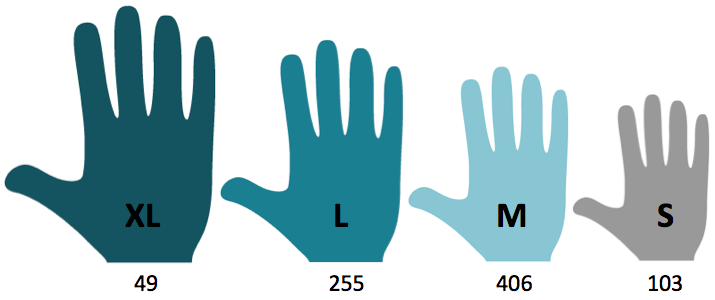
\includegraphics[width=0.8\textwidth]{pics/analysis/handsize.png}
      \caption{Handsize of all participants}
      \label{fig:handsize}
    \end{figure}
    \begin{table}[H]
      \centering
      \begin{tabular}{ c || c | c | c | c || c }
        \hline
        & {\bf Xtra Large} & {\bf Large} & {\bf Medium} & {\bf Small} & {\bf Total}\\ \hline
        {\bf Male} & 45 (9\%) & 200 (38\%) & 246 (47\%) & 38 (7\%) & 529 \\
        {\bf Female} & 3 (1\%) & 54 (19\%) & 157 (56\%) & 64 (23\%) & 278 \\ \hline
      \end{tabular}
      \caption{Handsize and gender}
      \label{tab:HandsizeGender}
    \end{table}

    The problem with using data being a subjective classification by the respondents, it is not known if the classification is correct. On the other side, what is a correct classification? The hand size of the respondents are not used for further analysis because of the difficulties of comparing the size selected by both genders against each other. If used, any results can not be guaranteed to be correct if including the hand size. The hand size property will are not being used further in this research.

    In the survey, both the subjective classification of the screen size as well as the height and width in pixels were collected. Classification of screen sizes is troublesome due to the various screen sizes and resolutions across different devices. Smartphones operating on Android are known to have a high variation in screen resolutions while Apple have created their devised with a smaller and fixed number of different screens. The physical size of a mobile screen is not correlated with the pixel size because a pixel is not a physical measure due to resolution, hence being troublesome to obtain the correct screen size. 

    Besides screen size and pixels, the respondents were asked for the mobile operating system on the device used. As a result of {\it Apple} having standardized the screen of their devices makes it possible to obtain the physical size of the screen for respondents using a iPhone for answering the survey. Figure \ref{fig:iphonescreenresolutions} is the complete list of the devices provided by Apple and the corresponding size in inches. 

    \begin{figure}[H]
      \centering
      \subfigure[iPhone 3.5"]{
        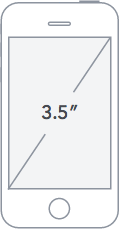
\includegraphics[scale=0.45]{pics/analysis/iphone35.png}
        \label{fig:iphone35}
      }
      \subfigure[iPhone 4"]{
        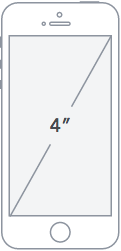
\includegraphics[scale=0.45]{pics/analysis/iphone4.png}
        \label{fig:iphone4}
      }
      \subfigure[iPhone 4.7'']{
        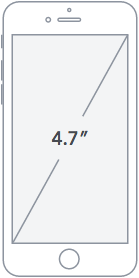
\includegraphics[scale=0.45]{pics/analysis/iphone47.png}
        \label{fig:iphone47}
      }
      \subfigure[iPhone 5.5'']{
        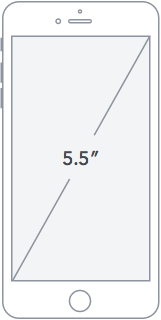
\includegraphics[scale=0.45]{pics/analysis/iphone55.png}
        \label{fig:iphone55}
      }

      \caption{iPhone screen resolutions}
      \label{fig:iphonescreenresolutions}
    \end{figure}

    There are only four sized used by Apple mobile devices as illustrated in Figure \ref{fig:iphonescreenresolutions}. In the dataset, there are only obtained the pixel sizes of the devices. For the devices running on iOS, four different types were observed in the dataset. The respondents' classification of the screen sizes, as well as the pixel size, are summarized in table \ref{fig:iphoneScreenDist} for all respondents using an iPhone.

    \begin{figure}[H]
      \centering
      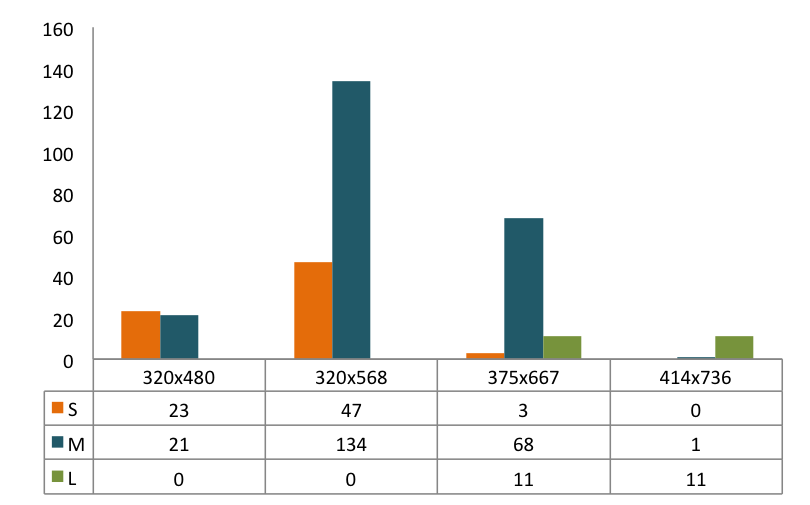
\includegraphics[scale=0.75]{pics/analysis/IphoneScreenDist.png}
      \caption{iPhone screensize distribution}
      \label{fig:iphoneScreenDist}
    \end{figure}

    To be able to evaluate the provided classification from the respondents, the Apple devices are classified according to what this research defines as a small, medium and big screen. The classifications are listed in Table \ref{tab:iphonescreen} with the corresponding device and pixel sizes. To be able to evaluate the provided classification from the respondents, the Apple devices are classified according to what this research defines as a small, medium and big screen. The classifications are listed in Table \ref{tab:iphonescreen} with the corresponding device and pixel sizes. When comparing Figure and \ref{fig:iphoneScreenDist} and Table \ref{tab:iphonescreen}, the respondents agree on the size to some extent. When looking at the number of respondents, only 40\% of the respondents used an iPhone, making the provided data for each screen type hard to use for further analysis. 

    \begin{table}[H]
      \centering
      \begin{tabular}{ l | l | l | l }
        \hline
        {\bf Iphone Model}  & {\bf Resolution (px)} & {\bf Inches} & {\bf Size} \\ \hline
        iPhone 2G, 3G, 3GS, 4, 4s  &  320 $\times$ 480  &  3.5'' & S\\
        iPhone 5, 5s        &  320 $\times$ 568  &  4'' & M \\
        iPhone 6            &  320 $\times$ 568, 375 $\times$ 667  &  4.7'' & M/L \\
        iPhone 6 Plus       &  375 $\times$ 667, 414 $\times$ 736  &  5.5'' & L \\ \hline        
      \end{tabular}
      \caption{iPhone screensizes}
      \label{tab:iphonescreen}
    \end{table}

    Based on the classification of the screen size on Apple devices, it can be used for evaluating respondent's ability to classify what this research defines as a small, medium or big screen. The problem with the rest of the respondents not using Apple products is that there is no fixed standard for screen sizes, making it impossible to predict the physical size by knowing the pixels. Since the majority of the respondents were using an Android device (58\%), making it unlikely of being able to classify the screen sizes correctly. The 40\% of the devices being an iPhone was possible with some uncertainty to classify, but the size of the dataset are too small for getting any results. Either being an Android or iOS device, it can neither be guaranteed to be correctly classified. It is therefore decided to not include any results using the screen size. 